\documentclass[11pt]{article}

\usepackage{fullpage}
\usepackage{graphicx}
\usepackage{tikz}
\usepackage{ulem}
\usepackage{array}
\newcolumntype{$}{>{\global\let\currentrowstyle\relax}}
\newcolumntype{^}{>{\currentrowstyle}}
\newcommand{\rowstyle}[1]{\gdef\currentrowstyle{#1}%
  #1\ignorespaces
}

\usetikzlibrary{shapes}

\renewcommand{\baselinestretch}{1.0}
\newcommand\tab[1][1cm]{\hspace*{#1}}
\usepackage{amsmath,amsthm,amssymb,amsfonts} % Typical maths resource packages
%\usepackage{graphicx}                 % Packages to allow inclusion of graphics
%\usepackage{color}                    % For creating coloured text and background
%\usepackage{multicol}
%\usepackage[all]{xy}

\oddsidemargin 0cm
\evensidemargin 0cm

%\newtheorem{theorem}{Theorem}[section]
%\newtheorem{proposition}[theorem]{Proposition}
%\newtheorem{corollary}[theorem]{Corollary}
%\newtheorem{lemma}[theorem]{Lemma}
%\newtheorem{remark}[theorem]{Remark}
%\newtheorem{definition}[theorem]{Definition}


% ******* User defined commands  *****************


\def\R{\mathbb{ R}}
\def\S{\mathbb{ S}}

\begin{document}
{\Large {\bf CS 222 Homework 7 [125 Points Total]}}  \\

\noindent \textbf{Online Submission via Canvas Only!} If you are not able to produce a PDF version, you can scan or take picture of your homework for submission. No paper submission will be accepted.\\

\noindent \textbf{Write your name on this sheet}. \textbf{No name or cover sheet will miss 2 points}




\begin{enumerate}
  \item (20 pts) Draw the undirected graph represented by the first adjacency matrix, and directed graph represented by the second adjacency matrix

    ~~~~~~~~$
    \begin{bmatrix}
        1 & 2 & 0 & 1 \\
        2 & 0 & 3 & 0 \\
        0 & 3 & 1 & 1\\
        1 & 0 & 1 & 0
    \end{bmatrix} ~~~~~~~~~~~~~~~~~~~~~~~~~~~~~~~~~~~~~~~~~~~~~~~~~~~~~~~~~~~~~~
   \begin{bmatrix}
        1 & 2 & 1 \\
        2 & 0 & 0 \\
        0 & 2 & 2
    \end{bmatrix}$\\
    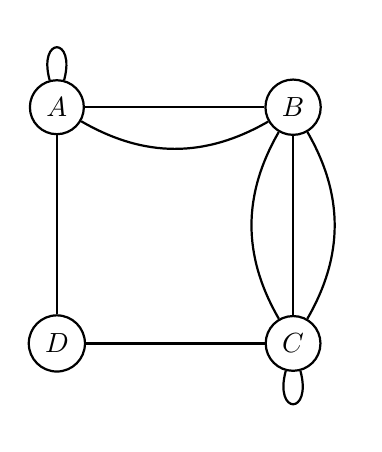
\begin{tikzpicture}[auto, node distance=3cm, every loop/.style={}, thick,main node/.style={circle,draw,font=\sffamily\Large\bfseries}]
      \node[circle, draw] (a) {$A$};
      \node[circle, draw] (b) [right of =a] {$B$};
      \node[circle, draw] (c) [below of =b] {$C$};
      \node[circle, draw] (d) [left of =c] {$D$};

      \path[every node/.style={font=\sffamily\small}]
        (a) edge [loop above] node {} (a)
             edge node {} (b)
             edge [bend right] node {} (b)
             edge node {} (d)
        (b) edge node {} (c)
             edge [bend left] node {} (c)
             edge [bend right] node {} (c)
        (c) edge [loop below] node {} (c)
             edge node {} (d)
        (d) 
         ;
    \end{tikzpicture} ~~~~~~~~~~~~~~~~~~~~~~~~~~~~~~~
    \begin{tikzpicture}[auto, node distance=4cm, every loop/.style={}, thick,main node/.style={circle,draw,font=\sffamily\Large\bfseries}]
      \node[circle, draw] (x) {$X$};
      \node[circle, draw] (y) [below right of =a] {$Y$};
      \node[circle, draw] (z) [below left of =a] {$Z$};
      
      \path[->,every node/.style={font=\sffamily\small}]
        (x) edge [loop above] node {} (x)
             edge node {} (y)
             edge [bend left] node {} (y)
             edge node {} (z)
        (y) edge node {} (x)
             edge [bend left] node {} (x)
        (z) edge node {} (y)
             edge [bend right] node {} (y)
             edge [loop above] node {} (z)
             edge [loop left] node {} (z)
         ;
    \end{tikzpicture}



  \item(40 pts) Given the a directed graph as shown below, answer the following questions:
  \begin{figure}[!ht]
  \begin{center}
  \includegraphics[height=6cm]{hw7-fig/hw7-q2.pdf}
  \end{center}
  \end{figure}


\begin{enumerate}
  \item (10 pts) What is the adjacency list representation of this graph? \\
    \begin{center}
      \begin{tabular}{|c|c|}
      \hline
      Initial Vertex & Terminal Vertexes \\
      \hline
      1 & 3  \\
      2 &     \\
      3 & 4 \\
      4 & 1,2 \\
      5 & 1,2\\
    \hline
    \end{tabular}
  \end{center}
    
  \item (10 pts) What is the adjacency matrix representation of this graph? \\
    \begin{center}
      $\begin{bmatrix}
        0 & 0 & 1 & 0 & 0 \\
        0 & 0 & 0 & 0 & 0 \\
        0 & 0 & 0 & 1 & 0 \\
        1 & 0 & 0 & 0 & 0 \\
        1 & 1 & 0 & 0 & 0 \\
      \end{bmatrix}$
    \end{center}
    
  \item (10 pts) Is the graph strongly connected? Why? \\
    \tab No because there is no directed path from 2 to 4 
    
  \item (10 pts) Is the graph weakly connected? Why? \\
    \tab Yes, if the graph is undirected then you can get from any point to any other point.
\end{enumerate}


\item (10 pts) Is there a undirected graph with degree sequence (3,2,2,2)? Why? \\
  \tab No, you can't have a full graph with an odd number of degrees.


\item (20 pts) Draw a directed graph to represent airline routes where every day there are four flights from Boston to Newark, two flights from Newark to Boston, three flights from Newark to Miami, two flights from Miami to Newark, one flight from Newark to Detroit, two flights from Detroit to Newark, three flights from Newark to Washington, two flights from Washington to Detroit, and one flight from Washington to Miami. \\
  \begin{center}
    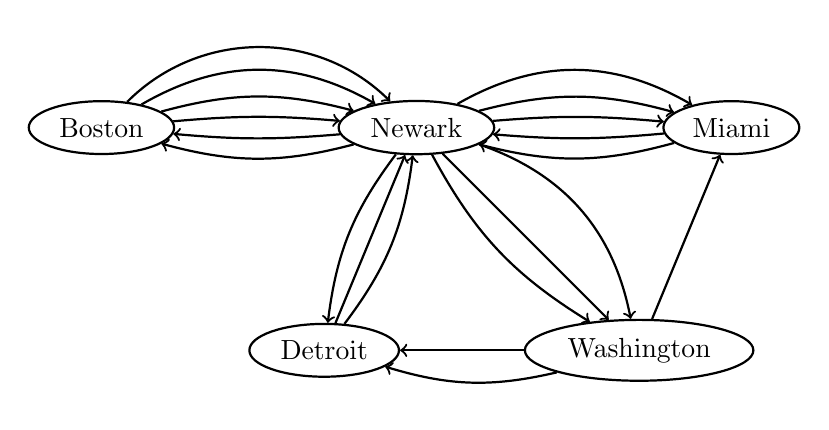
\begin{tikzpicture}[auto, node distance=4cm, every loop/.style={}, thick,main node/.style={circle,draw,font=\sffamily\medium\bfseries}]
      \node[ellipse,draw] (1) {Boston};
      \node[ellipse,draw] (2) [right of =1] {Newark};
      \node[ellipse,draw] (3) [right of =2] {Miami};
      \node[ellipse,draw] (4) [below right of =1] {Detroit};
      \node[ellipse,draw] (5) [below right of =2] {Washington};
    
      \path[->,every node/.style={font=\sffamily\Large}]
      (1) edge [bend left=5]node {} (2)
           edge [bend left=15] node {} (2)
           edge [bend left=30] node {} (2)
           edge [bend left=45] node {} (2)
      (2) edge [bend left=5] node {} (1)
           edge [bend left=15] node {} (1)
           edge [bend left=5] node {} (3)
           edge [bend left=15] node {} (3)
           edge [bend left=30] node {} (3)
           edge [bend right=15] node {} (4)
           edge node {} (5)
           edge [bend right=15] node {} (5)
           edge [bend left=30] node {} (5)
      (3) edge [bend left=5] node {} (2)
           edge [bend left=15] node {} (2)
      (4) edge node {} (2)
           edge [bend right=15] node {} (2)
      (5) edge node {} (4)
           edge [bend left=15] node {} (4)
           edge node {} (3)
       ;
    \end{tikzpicture}
  \end{center}

  \begin{itemize}
    \item (5 pts) In the graph you constructed, what is the in-degree and out-degree of the vertex for Detroit? \\
      \tab $d^-($Detroit$)=1 \tab d^+($Detroit$)=1$
  \end{itemize}


\item (30 pts) Determine Shortest Path from vertex 0 to all others using the Dijkstra’s Algorithm

\begin{figure}[!ht]
  \begin{center}
  \includegraphics[height=6cm]{hw7-fig/shortestpath.png}
  \end{center}
  \end{figure}

  \begin{center}
    \begin{tabular}{|$l|^l|^c|^c|^c|^c|^c|}
      \hline
      \rowstyle{\bfseries} Iteration & Init & 0 & 1 & 2 & 3 & 4 \\ \hline
      \textbf{Cur Node} & -- & 0 & 4 & 2 & 3 & 1 \\ \hline
      0 & \textbf{0} &  &  &  &  &  \\ \hline
      1 & $\infty$ & 5           &                & \textbf{5\textbf} &  &  \\ \hline
      2 & $\infty$ & 2           & \textbf{2}             &    &  &  \\ \hline
      3 & $\infty$ & $\infty$ & $1+2=3$ & \textbf{3} &  &  \\ \hline
      4 & $\infty$ & \textbf{1}           &                &    &  &  \\ \hline
    \end{tabular}
  \end{center}


 \end{enumerate}




\end {document}
